%%%%%%%%%%%%%%%%%%%%%%%%%%%%%%%%%%%%%%%%%%%%%%%%%%%%%%%%%%%%%%%%%%%%%%%
%      SEC. 1
%%%%%%%%%%%%%%%%%%%%%%%%%%%%%%%%%%%%%%%%%%%%%%%%%%%%%%%%%%%%%%%%%%%%%%%
\section{Introduction and structure of the thesis}

Passion and curiosity should always lie at the heart of the scientific practice, and that ought to be enough to define the value of a research effort~\cite{Weber1917,Shapin2015}. Time is the real arbiter of the significance of a piece of research, as many examples in the history of science show~\cite{Brush1967,Niss2008}\footnote{The Ising-Lenz model is one such example~\cite{Brush1967,Niss2008,Niss2004}. It was suggested by physicist Wilhelm Lenz to his doctoral student Ernst Ising to study phase transitions in ferromagnetic materials. Ising solved it analytically in 1D as part of his Ph.D. defense in 1925, but the solution for a 1D lattice did not show any phase transition. This apparent failure is thought to be the reason of Ising's decision to take a job outside academia. Almost 20 years later, Onsager solved the 2D version of the model and showed the possibility of phase transitions in the Ising-Lenz model. By the time Ising arrived in the USA in 1947, the Ising-Lenz model was already entering the canon of physics and, to his surprise, he was being asked if he was ``the Ising" of the ``Ising model".}.However, in these years of increasing mistrust towards scientific research and brewing doubts on the value of universities and research institutes~\cite{Biesta2002,Biesta2004,Santos2012}, it is worthwhile to try to place one's own work into the wider picture of one's own time. It is also a valuable exercise for the researcher, who sensibly progresses in the work by investigating one detail at a time, to spend a moment away from one's own graphs and equations and see their place in the wider perspective of the world outside the laboratory.\\
It is thus in this spirit that I propose to open the present work with a reflection on the challenges that the transportation industry faces at the closing of $21^{st}$ century's second decade. Against this background, in Chapter~1 \emph{thin-ply} laminates are introduced as a very promising material for innovative structural design and their main characteristics are discussed. The focus is then moved to the most renown quality of \emph{thin-ply} laminates, i.e. their ability to delay and even suppress onset and propagation of transverse cracking, and to discuss the modeling issues that this new material poses. Finally, a link is established with the growth of fiber/matrix interface cracks or, as very often called in the rest of the thesis, debonds. Chapter~2 opens with an introduction to the main concepts of Fracture Mechanics. The fiber/matrix interface crack is then discussed in detail, and previous analytical, computational and experimental studies available in the literature are reviewed. The modeling strategy adopted in this thesis is then presented and its implementation described. Finally, Chapter~3 provides a summary of the main results of this work, organized following the order of the publications reported in Part~II of the thesis. The first chapter is thus a journey of scales: we start from the challenges of an industrial sector, move to the structural requirements of its products, focus on a promising new material, and concentrate on understanding the mechanisms of damage initiation in it.

\section{Vision 2030: challenges of the next decade and beyond for the transportation industry}

The closing of the second decade of the $21^{st}$ century brings different challenges for the transportation industry, which will likely shape its development in the next decade and beyond. A brief review of the most relevant aspects is proposed here.

\begin{description}
\item[Climate action.] The issue of climate change is certainly one the ``hot" topic of today's public debate. A discussion of the merits of scientific understanding of climate change, public reception, media coverage and socio-political implications is out of the scope of the present work, but it is certainly one of the most relevant topic framing today's public discourse. Given that it is a high-divisive subject, no judgement on the validity of the claims of one side or the other is proposed here, as sufficient space can not be devoted to a thorough analysis of the problem. What is acknowledged here is the emergence of concerted efforts at the institutional level (companies, city administrations, regional governments, sovereign states) to rule into and provide control mechanisms to limit the emission of carbon dioxide, i.e. $CO_{2}$. The evidence of this shift in public policy is exemplified in Figure~\ref{chap1:fig:climatedealssignataries} and Figure~\ref{chap1:fig:greenfundpledges}.\\ Figure~\ref{chap1:fig:climatedealssignataries} reports the evolution over time of the number of signatories of three representative deals on climate action. The selected deals are: the Vienna Convention for the Protection of the Ozone Layer, first signed in 1985 and committing signatories to the reduction of chlorofluorocarbons; the United Nations Framework Convention on Climate Change (UNFCCC), initially agreed in 1992 with the aim of managing the increase in greenhouse emission in order to avoid dangerous interferences with the climate; the Kyoto Protocol, signed in 1997 as an extension of the UNFCCC and according to which adhering countries pledge to reduce greenhouse emissions to prevent climate change. Figure~\ref{chap1:fig:climatedealssignataries} shows how the majority of countries have ratified these deals over time, reaching an almost unanimous agreement on the need of coordinated action towards the issues of climate change.

\begin{figure}[!h]
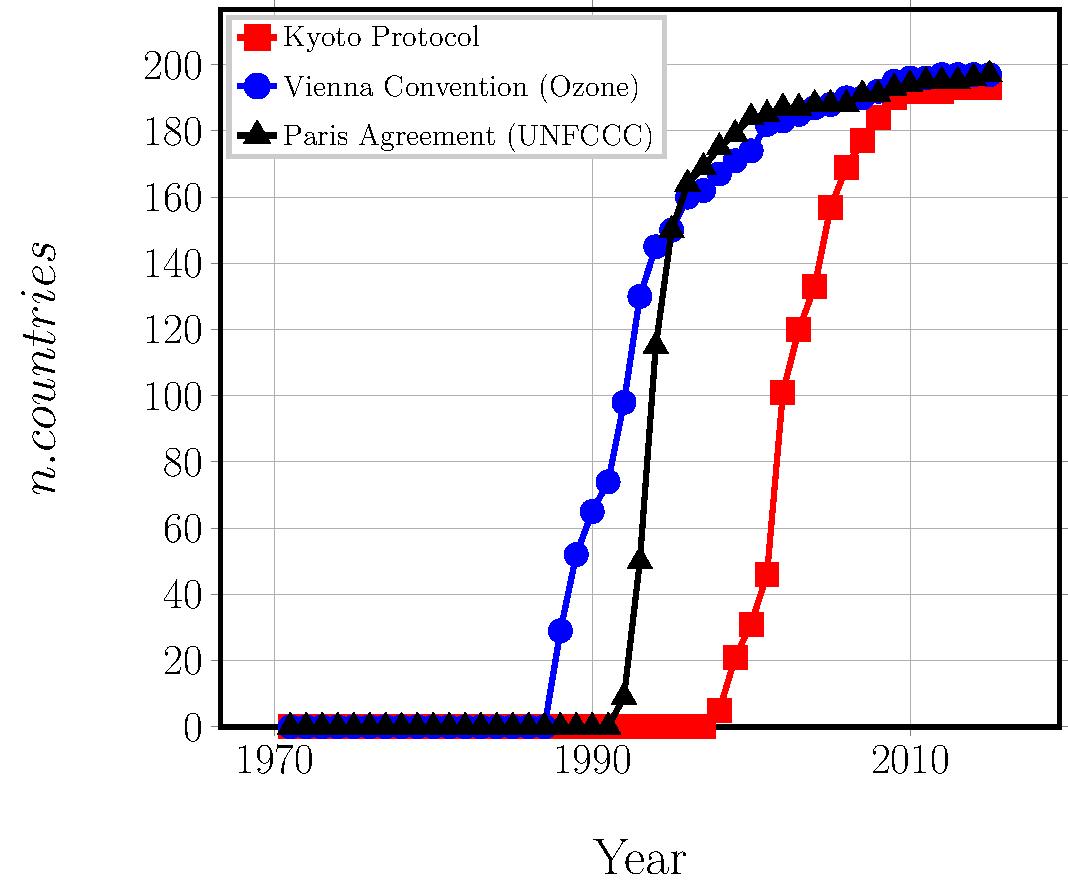
\includegraphics[width=0.9\textwidth]{pics/climate-deals-signataries.pdf}
\caption{Number of signing countries over time for selected deals on climate. Source: UNCTAD Development and Globalization: Facts and Figures (2016). United Nations Conference on Trade and Development. Available at \href{https://stats.unctad.org/Dgff2016/DGFF2016.pdf}{https://stats.unctad.org/Dgff2016/DGFF2016.pdf} (last access: September 26, 2019).}\label{chap1:fig:climatedealssignataries}
\end{figure}

Figure~\ref{chap1:fig:greenfundpledges} shows the 10 highest contributions to the Green Climate Fund, which aims to support projects in developing countries focusing on reduction of greenhouse gas emissions and climate adaptation. The commitment to this effort of industrialized countries is evident in Figure~\ref{chap1:fig:greenfundpledges}. It is thus apparent from Figure~\ref{chap1:fig:climatedealssignataries} and Figure~\ref{chap1:fig:greenfundpledges} that a shift in public attitude and policy towards the issues of climate change has been under way in the last decades. This shift in turn has been materialized in the form of international agreements on climate action, which have led to the introduction of novel regulations aimed at containing the emission of $CO_{2}$ and other pollutants into the atmosphere and biosphere at large.

\begin{figure}[!h]
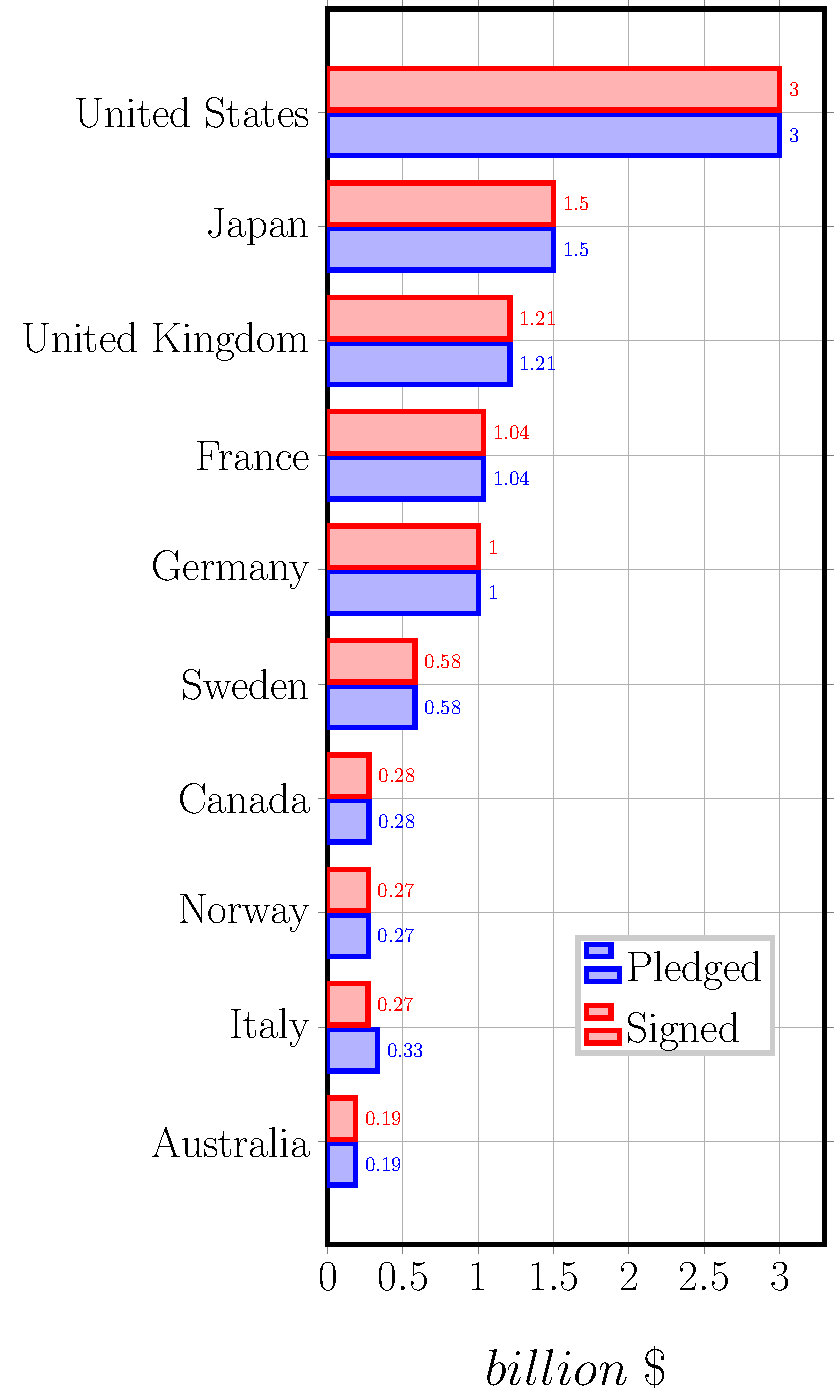
\includegraphics[height=0.75\textheight]{pics/green-fund-pledges.pdf}
\caption{Pledged and signed contributions to the Green Climate Fund of the 10 countries with the highest signed contributions. Source: Green Climate Fund, available at \href{https://www.greenclimate.fund/how-we-work/resource-mobilization}{https://www.greenclimate.fund/how-we-work/resource-mobilization} (last access: September 21, 2019).}\label{chap1:fig:greenfundpledges}
\end{figure}

It is interesting to understand the impact of this shift on the transport industry by looking at some representative data of its $CO_{2}$ emissions. In Figure~\ref{chap1:fig:co2transportshare} the share of total $CO_{2}$ emissions is reported for some selected countries. The first observation is that the role of the transport industry as a source of $CO_{2}$ has been increasing over the years. Today it accounts for around $30\%$ of total emissions in large mature economies such as the United States and the European Union, around $20\%$ of Japan's emissions and $10\%$ of China's.

\begin{figure}[!h]
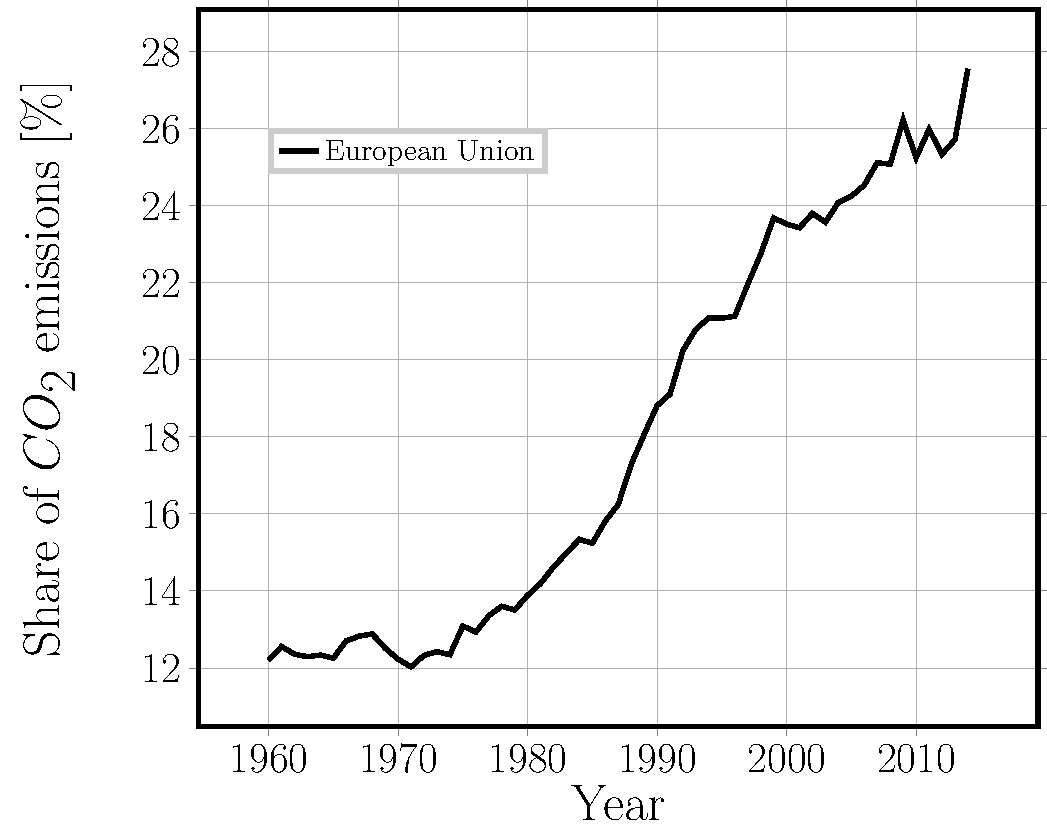
\includegraphics[width=0.9\textwidth]{pics/co2transportshare.pdf}
\caption{Share of total $CO_{2}$ emissions due to the transport sector over time for selected countries. Source: International Energy Agency (IEA) via The World Bank, available at \href{http://data.worldbank.org/data-catalog/world-development-indicators}{http://data.worldbank.org/data-catalog/world-development-indicators} (last access: September 21, 2019).}\label{chap1:fig:co2transportshare}
\end{figure}

A second perspective on the problem in provided in Figure~\ref{chap1:fig:co2transportabsolute}, where the evolution of $CO_{2}$ total emissions (in absolute terms) for selected world geographical entities is compared with that of international transport. Interestingly, the emissions of the latter has been comparable in the last 50 years to those of the African continent as a whole.

\begin{figure}[!h]
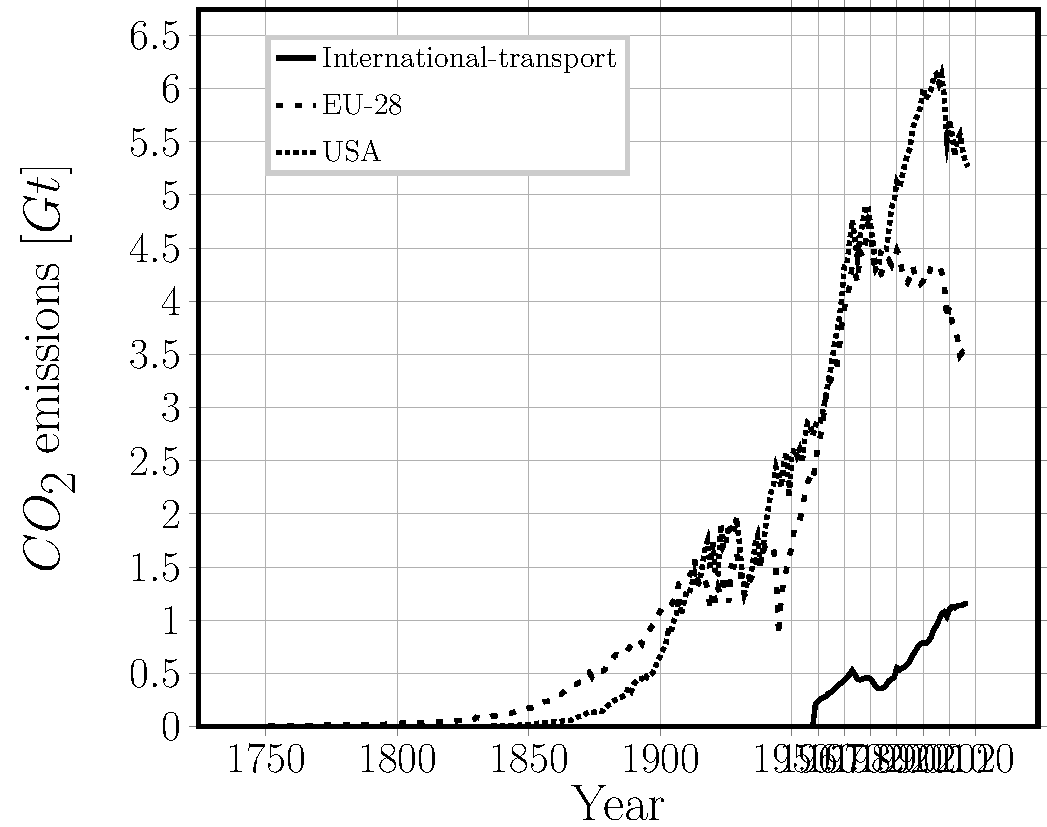
\includegraphics[width=0.9\textwidth]{pics/co2transportabsolute.pdf}
\caption{Total $CO_{2}$ emissions due to transport over time, compared with selected geographical entities. Source: The Global Carbon Project, available at \href{https://www.globalcarbonproject.org/}{https://www.globalcarbonproject.org/} (last access: September 21, 2019).}\label{chap1:fig:co2transportabsolute}
\end{figure}

It is thus clear from Figure~\ref{chap1:fig:co2transportshare} and Figure~\ref{chap1:fig:co2transportabsolute} that the transport sector plays a prominent role in the emission of $CO_{2}$ and other pollutants into the biosphere. It is, and will be, strongly affected by the emphasis on climate change that currently characterizes international public policy. Stricter standards on emissions are planned or expected in several parts of the world and the transport industry, currently one the biggest emitter, needs to innovate to adapt to this change.

\item[Increased competitiveness.] During the last couple of decades, the arrival of new players and the introduction of new business models have increased competitiveness in the transport sector and favored a downward pressure on prices. Several examples exist. In civil aviation, the diffusion of low-cost carriers such as Ryanair$^{TM}$, easyJet$^{TM}$ and Norwegian$^{TM}$, which offer very (and sometimes even extreme) low rates by drastically reducing the number of ancillary service comprised in the ticket price, which are then offered as pay-as-you-go additional services. The space sector has seen the arrival of a number of private actors which are developing or are already proposing on the market low-Earth launching technologies significantly cheaper than market incumbents. In the car industry, ride-sharing (such as BlaBlaCar$^{TM}$) and ride-hailing services (like Uber$^{TM}$ and Lyft$^{TM}$) are leading to a change in the importance of car ownership and, thus, in the role of car manufacturers.

\begin{figure}[!h]
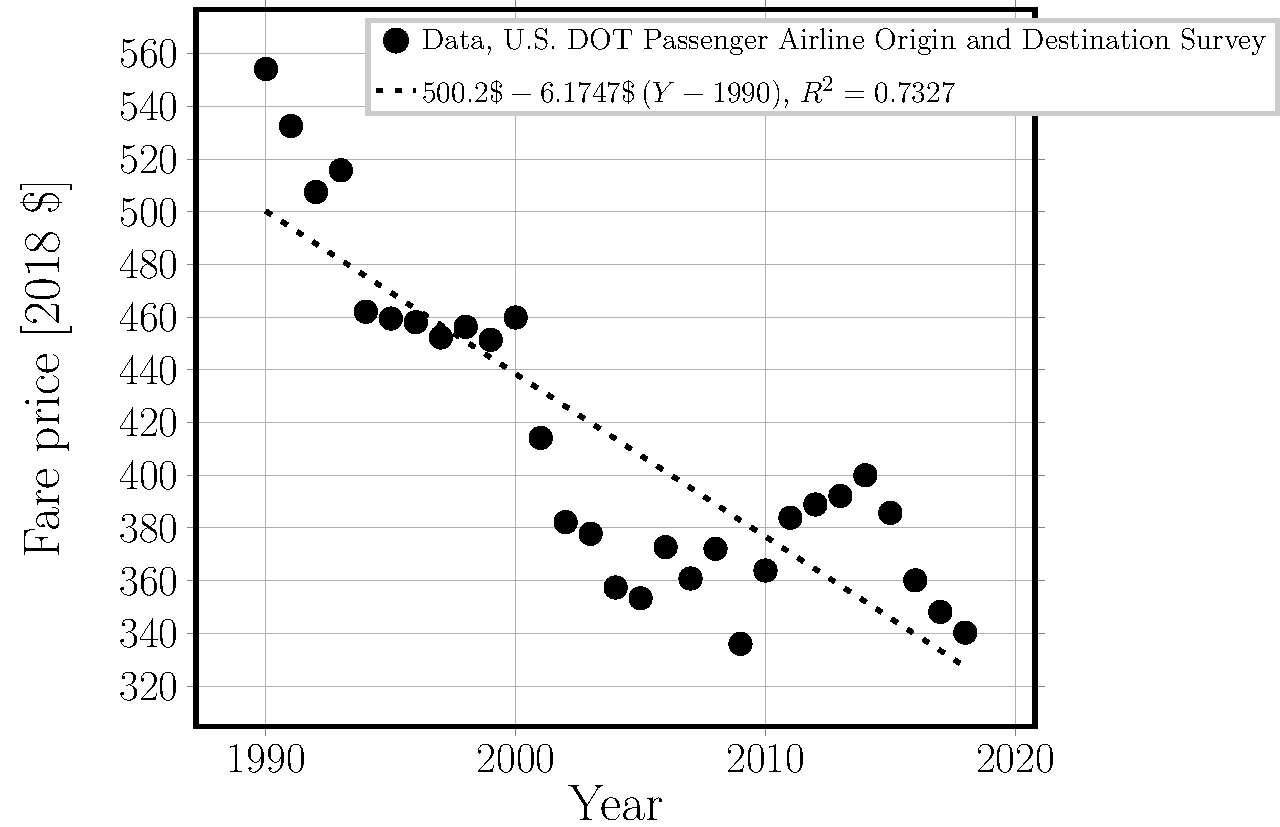
\includegraphics[width=0.9\textwidth]{pics/airlinefarecost.pdf}
\caption{Average airline fare in the United States over the years, prices in $2018\ \$$. Source: , available at \href{}{} (last access: , 2019).}\label{chap1:fig:airlinefarecost}
\end{figure}

Two representative examples of the reduction of prices over time in the transport industry are shown in Figure~\ref{chap1:fig:airlinefarecost} and in Figure~\ref{chap1:fig:spacetravelcost}. In Figure~\ref{chap1:fig:airlinefarecost}, the evolution of fare prices (expressed in 2018 US \$) over the past three decades in the United States is reported. A clear downward trend is observable and a linear regression of the data provides a negative slope with a $R^{2}$ coefficient of $0.7327$. Figure~\ref{chap1:fig:spacetravelcost} presents the unit cost (expressed in 2018 US \$) of payload for several different launch system with respect to time. Three systems are in particular highlighted: the Vanguard, the first one in history; the Space Shuttle, for introducing the concept of launch system reusability; the Falcon Heavy, for bringing to the market a privately managed reusable launcher system. Albeit with some scatter, it is possible to observe a downward trend of prices. A linear regression of the logarithm of price with respect to time provides an estimate of the year-on-year price decrease at around $3\%$, i.e. a $30\%$ every decade.

\begin{figure}[!h]
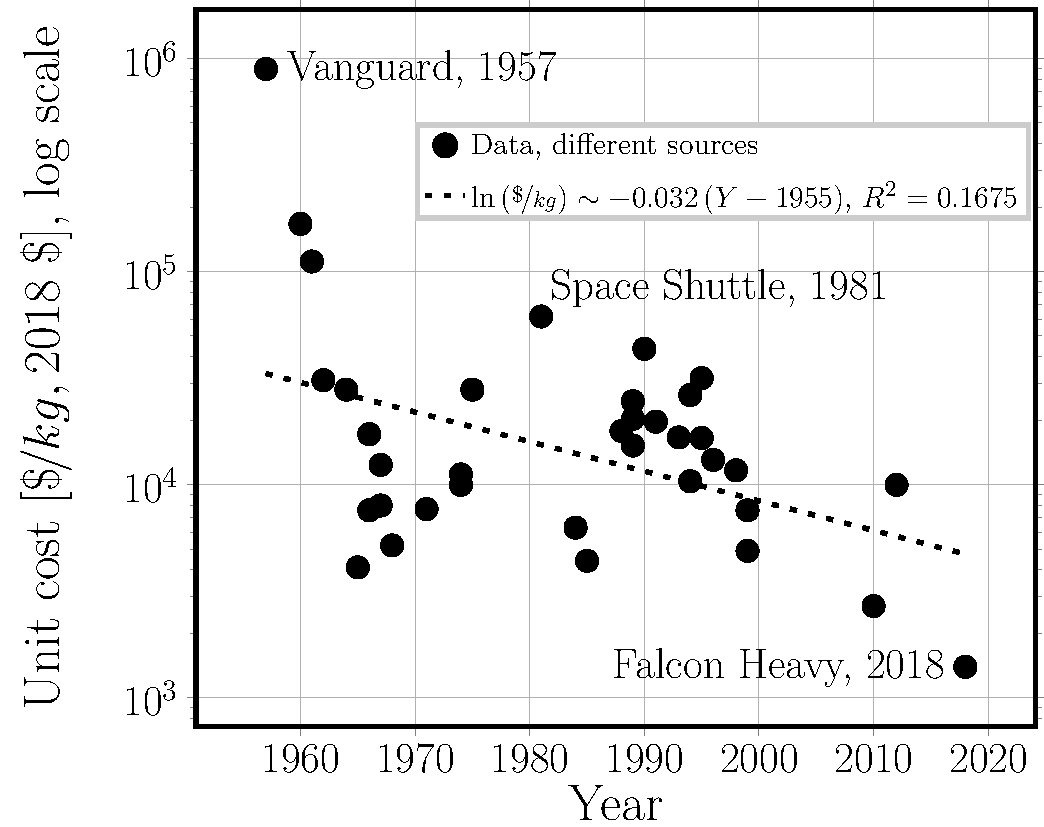
\includegraphics[width=0.9\textwidth]{pics/spacetravelcost.pdf}
\caption{Evolution of unit cost of payload for different launching over time, prices in $2018\ \$$. Source: , available at \href{}{} (last access: , 2019).}\label{chap1:fig:spacetravelcost}
\end{figure}

\item[Safety and crashworthiness.] Strict requirements on vehicles safety and crashworthiness are not a novelty of the 2010's, as legislation has been built over the years to create a system of control and verification to ensure that vehicles' structures are reliable under normal operating life as well as exceptional conditions. However, the recent crashes of the two Boeing 737 MAX 8 planes of Lion Air in Indonesia~\cite{aviationSafety2018} and of Ethiopian Airlines in Ethiopia~\cite{aviationSafety2019} have put the issue of safety and crashworthiness back into the spotlight, as the cause of the crashes was a technical glitch in the automatic guidance and control system. Thus, although the problem is one of software development and control system engineering, it calls for a revision of current practices of oversight and certification. For the structural designer, requirements of safety and crashworthiness translate into a thorough understanding of structural failure mechanisms, and thus of the evolution of damage in the materials employed.

These issues are framing the evolution of the transport industry over the next decade, particularly in technological terms. Their requirements are often incompatible and current solution represents often a trade-off between them. Renewed efforts are thus devoted to the development of materials that could satisfy at the same time the needs of sustainability, price reduction and structural safety.

\section{\textit{Thin-ply} laminates and the \textit{spread tow} technology}

A very promising material introduced into the market by the composite industry in recent times is the so-called \emph{thin-ply} laminate, result of a series of advancements in the \textit{spread tow technology}. Conventionally, fibers are produced as bundles or \textit{tows} comprising $12/24k$ filaments; tows are then stacked together and impregnated in order to produce prepreg plies. At the heart of the \textit{spread tow technology} lies the idea of opening or \textit{spreading} such tows to create thinner and wider tapes, to be then used in the production of unidirectional (UD) prepregs or woven fabrics, as schematically depicted in Figure~\ref{chap1:fig:spreadtowtech}.

\begin{figure}[!h]
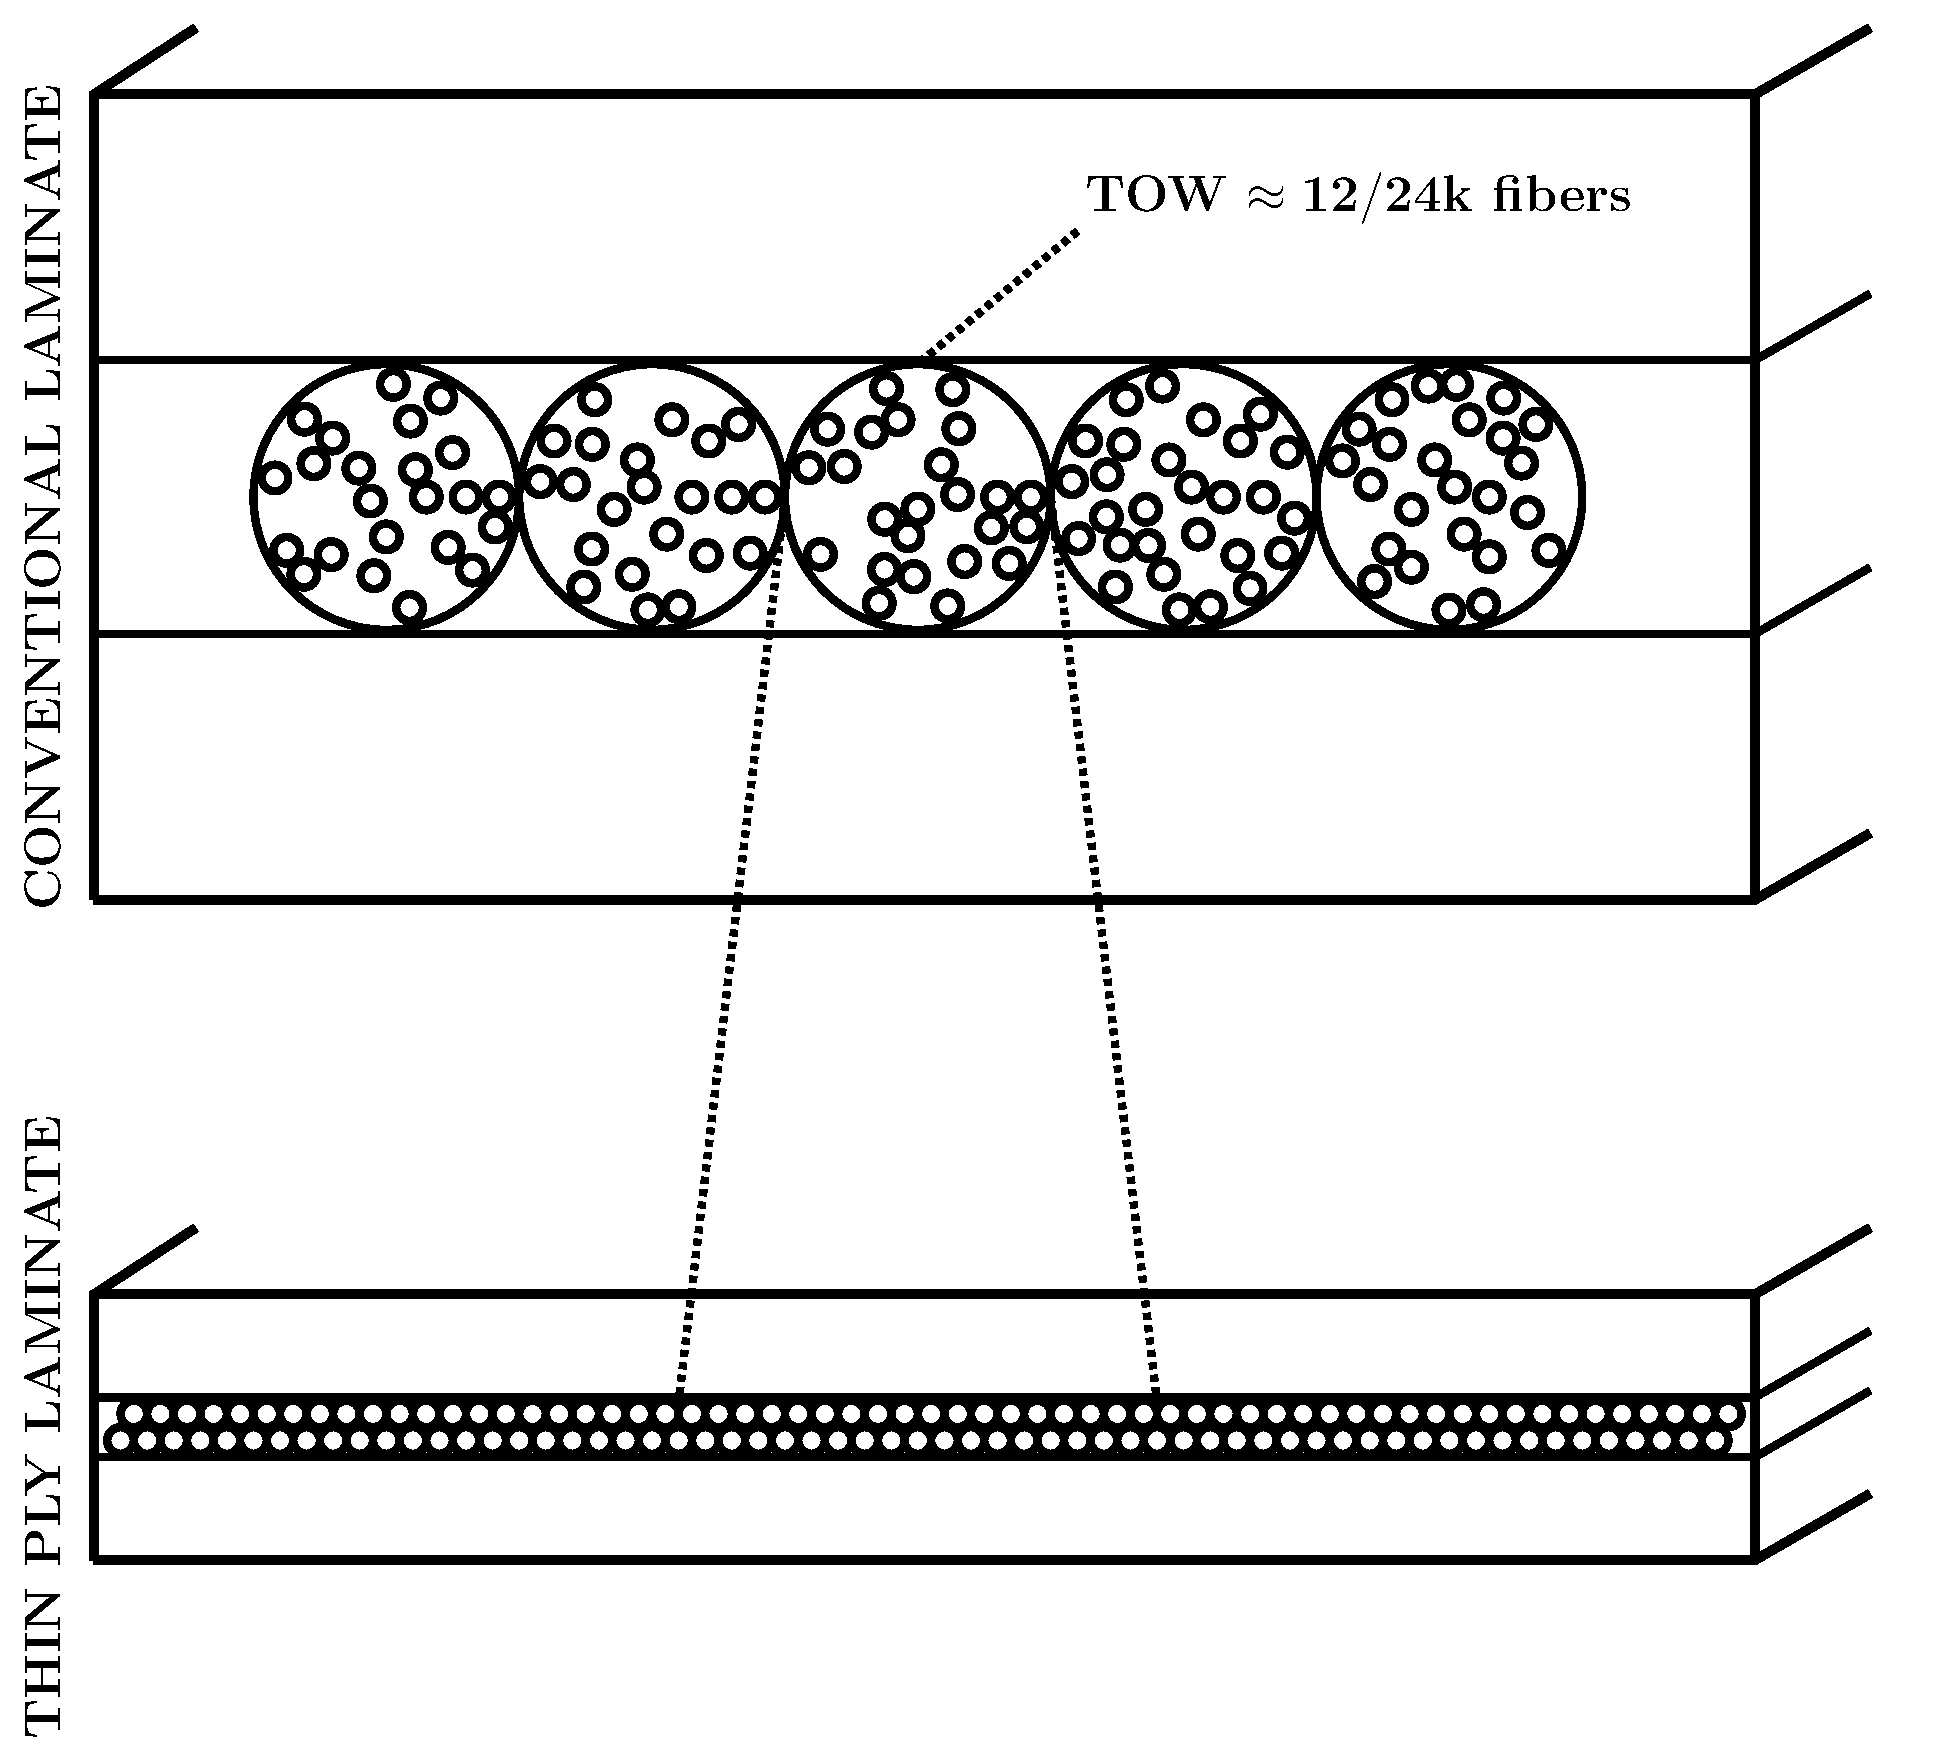
\includegraphics[width=0.75\textwidth]{pics/spread-tow-tech.pdf}
\caption{Schematic of the difference between laminates with conventional prepreg plies and \emph{thin-ply} laminates, issued from the \textit{spread tow technology}.}\label{chap1:fig:spreadtowtech}
\end{figure}

First attempts to turn the idea into practice date back to the 1970's~\cite{spreadtowpatent:1974}, when a Venturi injector opposite to the pulling direction of fibers was employed to split the tow. Other methodologies were then proposed, among others: acoustic vibrations in air generated by a speaker or similar apparatus below the tow~\cite{spreadtowpatent:1991}; mechanical separation by means of cylindrical rollers~\cite{spreadtowpatent:1992}; the use of expandable elastic bands (or tubes) mounted on a rotating drum~\cite{spreadtowpatent:2000}; electrostatic separation employing a corona discharge~\cite{spreadtowpatent:1993}. Nonetheless, they all suffered from a number of drawbacks: among the most critical, widespread breakages of fibers and deterioration of fiber surface properties, in particular wettability. A breakthrough arrived at the end of the 1990's, with the publication in 1997 of a contribution to the $42^{nd}$ SAMPE USA conference detailing a new spreading technique~\cite{Intro:KawabeTomodaMatsuo:1997} developed at the Industrial Technology Center in Japan's Fukui Prefecture. The technique, further improved in subsequent years~\cite{spreadtowpatent:2003,Intro:Kawabe:2008,Intro:SasayamaTomoda:2009}, is based on the combined use of focused air jets and a vacuum pump perpendicular to the pulling direction of fibers. Thanks to its capacity to avoid fiber breakage and fiber surface property loss, the technology has been applied on industrial scale to produce high-quality extremely thin fiber-reinforced prepreg plies. Only a few manufacturers exist today that produce \emph{thin-ply} laminates, among them North Thin Ply Technology (NTPT)~\cite{ntpt} in Switzerland (founded in 2001), Oxeon~\cite{oxeon} in Sweden (founded in 2003), Chomarat~\cite{chomarat} in France, Sakai Ovex~\cite{sakai} in Japan. The technology is now reaching a mature stage and proposals have been made to use \emph{thin-ply} laminates in primary load-carrying structural in safety critical applications such as Low-Earth Orbit (LEO) satellites~\cite{Moon2011}, airplane wings~\cite{Kim2017}, pressure vessels for cryogenic fuels~\cite{McCarville2018}, re-usable space launchers~\cite{Kopp2017}.\\
Probably the first assessment of the mechanical performance of \emph{thin-ply} laminates was published by the developers of the \emph{spread tow} technology themselves in 2004 in the Journal of the Japan Society for Composite Materials~\cite{sasayamaJSCM2004}. They studied the effect of ply thickness on first-ply failure in quasi-isotropic carbon fiber laminates under static tensile loading and observed an increase of the value of the stress at first ply failure.  Soon after, K. Yamaguchi and H. T. Hahn~\cite{Yamaguchi2005} reported that, in cross-ply laminates subjected to static tensile loading, no transverse crack and no delamination was observed in the \emph{thin-ply} specimen. According to the authors, fatigue behavior was also improved in \emph{thin-ply} laminates: the rate of growth of micro-cracks density was slowed and no transverse-crack induced delamination appeared even after $10^{6}$ cycles. The same year (2005), two contributions~\cite{TsaiICCM2005,Tsai2005} by S. Tsai and collaborators confirmed these observations. They tested cross-ply and quasi-isotropic laminates in simple static tension, static open hole tension and fatigue, and observed the suppression of micro-cracking and transverse-cracking induced delaminations. A number of experimental studies on \emph{thin-ply} laminates then followed, following the increasing interest from industry and responding to the need of the latter to characterize and standardize the properties of this new type of composite material. A comprehensive mechanical characterization of carbon fiber \emph{thin-ply} laminates is described in~\cite{Sihn2007}. Here the authors compare the results of different tests between two different types of laminates, both made with the same number of ply and with the same \emph{spread-tow} but with different effective thicknesses of the layers: the first type, namely the ´´thick" laminate, has layers made up by 5 plies for a thickness of $200\ \mu m$; the second, namely the ´´thin" laminate, has layers made up by only 1 ply for a thickness of $40\ \mu m$.


\end{description}
